\begin{frame}{Fluidos compresibles e incompresibles}
\justifying
Si es que las consideraciones físicas (termodinámicas y geométricas) no cambian la densidad del fluido, este fluido es incompresible.
Para el caso de un fluido compresible:
\begin{figure}[H]
\centering
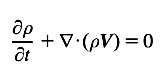
\includegraphics[scale=0.4]{Section_Files/S2-imagenes-Manuel/14.png}
\caption{Ecuación de continuidad.}
\end{figure}
Si el fluido es incompresible, tenemos:
\begin{figure}[H]
\centering
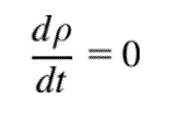
\includegraphics[scale=0.2]{Section_Files/S2-imagenes-Manuel/15.png}
\end{figure}
\begin{figure}[H]
\centering
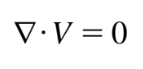
\includegraphics[scale=0.3]{Section_Files/S2-imagenes-Manuel/16.png}
\caption{Por lo cual el gradiente de velocidad es cero, lo cual significa que el fluido no presenta un cambio de volúmen (condición de incompresibilidad).}
\end{figure}
\end{frame}

\begin{frame}{Fluidos compresibles e incompresibles - ejercicio}
\begin{figure}[H]
\centering
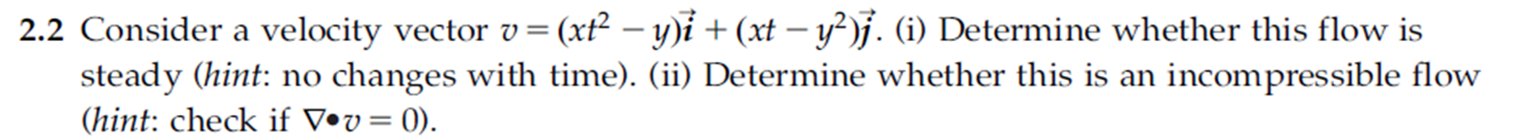
\includegraphics[scale=0.4]{Section_Files/S2-imagenes-Manuel/17.png}
\end{figure}
{\tiny Biomedical engineering por David Rubestein}
\end{frame}